\section{Performance Analysis}
\label{sect:performance}

The following analysis used a prototype of the \ulfm proposal based on
the development trunk of Open MPI~\cite{gabriel04:_open_mpi} (r26237).
The test results presented were gathered from the Smoky system at Oak
Ridge National Laboratory. Each node contains four quad-core 2.0~GHz AMD
Opteron processors with 2 GB of memory per compute core. Compute nodes
are connected with gigabit Ethernet and InfiniBand. Some shared-memory
benchmarks were conducted on Romulus, a $6\times8$-core AMD Opteron 6180
SE with 256GB of memory (32GB per socket) at the University of Tennessee.

\begin{figure}[ht]
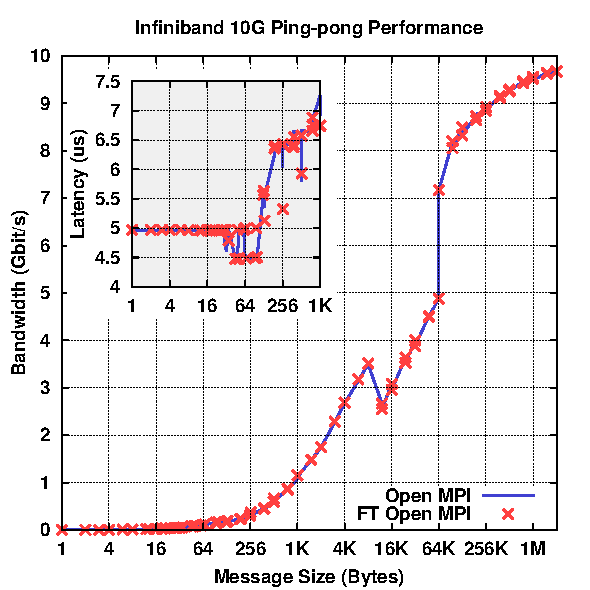
\includegraphics[width=.49\textwidth]{figures/np-ibsmoky}
\hfill
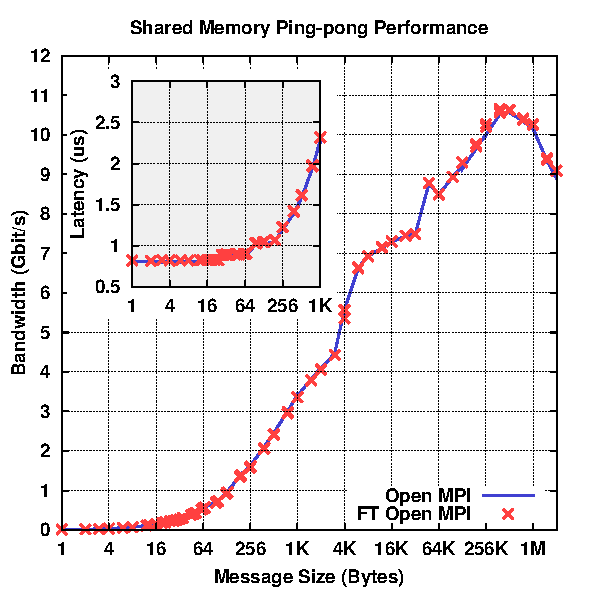
\includegraphics[width=.49\textwidth]{figures/np-smsmoky}
\caption{Netpipe Latency and Bandwidth Impact of Enabling Fault Tolerance Support (on Smoky)\label{fig:netpipe}.}
\end{figure}

\begin{table}%\vspace{-.4cm}
\begin{center}\sf\scriptsize
\begin{tabular}{|l||r|r||r|r||r|}
\multicolumn{6}{c}{1-byte Latency (microseconds) (cache hot)} \\
\hline
\cellcolor[gray]{0.7}\textbf{Interconnect}  & \cellcolor[gray]{0.7}\textbf{Vanilla}   & \cellcolor[gray]{0.7}\textbf{Std. Dev.} &
\cellcolor[gray]{0.7}\textbf{FT}            & \cellcolor[gray]{0.7}\textbf{Std. Dev.} & \cellcolor[gray]{0.7}\textbf{Difference} \\
\hline
\cellcolor[gray]{0.9}Shared Memory &  0.8008 & 0.0093 &  0.8016 & 0.0161 &  0.0008 \\
\cellcolor[gray]{0.9}TCP           & 10.2564 & 0.0946 & 10.2776 & 0.1065 &  0.0212 \\
\cellcolor[gray]{0.9}OpenIB        &  4.9637 & 0.0018 &  4.9650 & 0.0022 &  0.0013 \\
\hline
\multicolumn{6}{c}{Bandwidth (Mbps) (cache hot)} \\
\hline
\cellcolor[gray]{0.7}\textbf{Interconnect}  & \cellcolor[gray]{0.7}\textbf{Vanilla}   & \cellcolor[gray]{0.7}\textbf{Std. Dev.} &
\cellcolor[gray]{0.7}\textbf{FT}            & \cellcolor[gray]{0.7}\textbf{Std. Dev.} & \cellcolor[gray]{0.7}\textbf{Difference} \\
\hline
\cellcolor[gray]{0.9}Shared Memory &  10,625.92 &  23.46 &  10,602.68 & 30.73 & -23.24 \\
\cellcolor[gray]{0.9}TCP           &   6,311.38 &  14.42 &   6,302.75 & 10.72 &  -8.63 \\
\cellcolor[gray]{0.9}OpenIB        &   9,688.85 &   3.29 &   9,689.13 &  3.77 &   0.28 \\
\hline
\end{tabular}
\end{center}
\caption{Standard Deviation of the NetPIPE results (on Smoky).\label{tab:netpipe}}%\vspace{-.8cm}
\end{table}

The NetPIPE benchmark (v3.7) was used to assess the 1-byte latency and
bandwidth impact of the modifications necessary for the \ulfm support in
\ompi. We compare the vanilla version of \ompi (r26237) with the \ulfm
enabled version on Smoky (labelled as FT). Figure~\ref{fig:netpipe} compares the
bandwidth and latency achieved by these two builds of \ompi. As can be
observed, for the entire range of message sizes, the performance
difference is insignificant, either when using the Infiniband network
transport, or with the most stressful shared-memory transport.
Table~\ref{tab:netpipe} presents the standard deviation across 100 runs,
and further highlights the fact that the differences in performance are
not only well below the noise limit, but that the standard deviation
difference is negligible, thus proving the performance stability and
lack of impact.


\begin{figure}[ht]
\begin{center}%\vspace{-.6cm}
 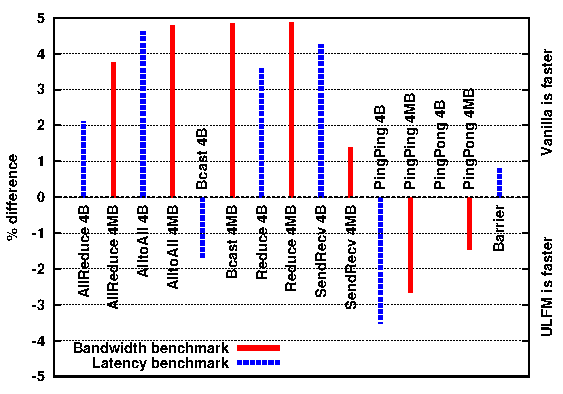
\includegraphics[width=.7\linewidth]{figures/IMB.pdf}%\vspace{-.4cm}
 \caption{The Intel MPI Benchmarks: relative difference
   between \ulfm and the vanilla Open MPI on shared memory
  (Romulus). Standard deviation $\approx$5\% on 1,000 runs.\label{fig:IMB}}%\vspace{-.6cm}
\end{center}
\end{figure}

The impact on shared memory systems, which are sensitive even to small
modifications of the MPI library, has been further assessed on the
Romulus machine -- a large shared memory machine -- using the IMB
benchmark suite (v3.2.3). As shown in Figure~\ref{fig:IMB}, the duration
difference of all the benchmarks (point-to-point and collective) remains
below 5\%, thus within the standard deviation of the implementation on
that machine.

To measure the impact of the prototype on a real application, we used the
Sequoia AMG benchmark\footnote{https://asc.llnl.gov/sequoia/benchmarks/\#amg}.
This MPI intensive benchmark is an Algebraic Mult-Grid (AMG) linear system
solver for unstructured mesh physics. A weak scaling study was conducted up to
512 processes following the problem \emph{Set 5}. In
Figure~\ref{fig:sequoia:bargraph}, we compare the time slicing of three main
phases (Solve, Setup, and SStruct) of the benchmark, with, side by side, the
vanilla version of the Open MPI implementation, and the \ulfm enabled one. The
application itself is not fault tolerant and does not use the features proposed
in \ulfm. The goal of this benchmark is to demonstrate that a careful
implementation of the proposed semantic does not impact the performance of the
MPI implementation, and ultimately leaves the behavior and performance
of legacy applications unchanged. The results show that the performance 
difference is negligible.

\begin{figure}[ht]
\centering
    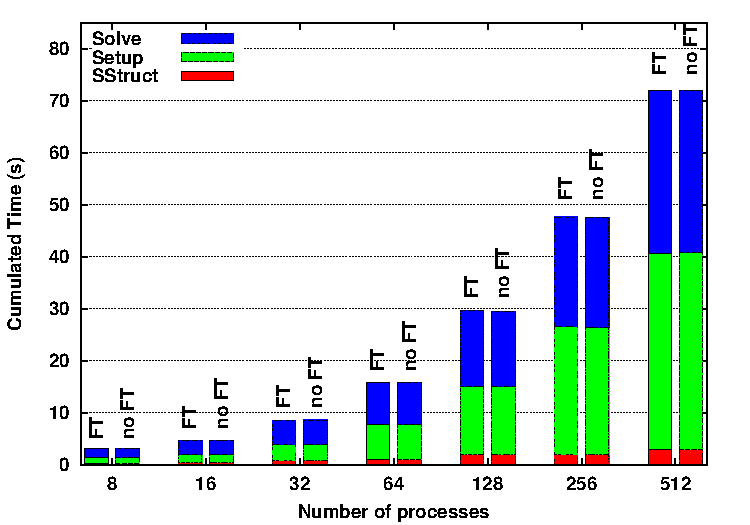
\includegraphics[width=.7\linewidth]{figures/bargraph.pdf}%\vspace{-.4cm}
    \caption{Comparison of the vanilla and \ulfm versions of Open MPI running
      Sequoia-AMG at different scales (Smoky).\label{fig:sequoia:bargraph}}
\end{figure}
\begin{figure}[ht]
\centering
    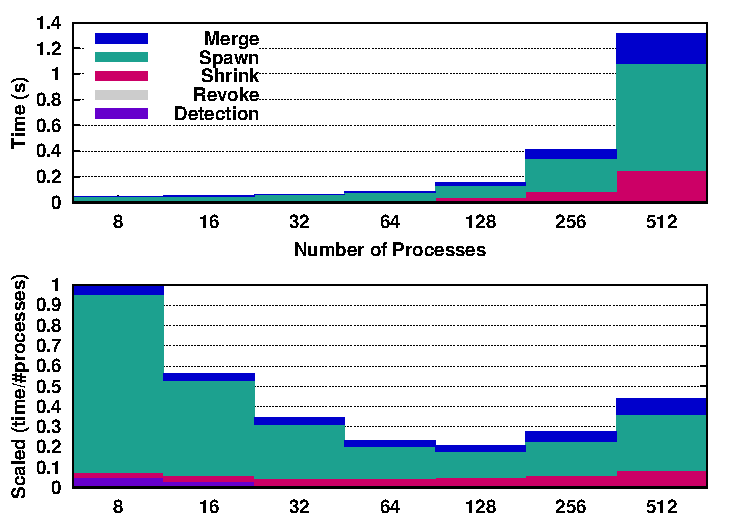
\includegraphics[width=.7\linewidth]{figures/repair.pdf}%\vspace{-.4cm}
    \caption{Evaluation of the Fault Injection Benchmark with full
      recovery at different scales (Smoky).\label{fig:frssj:scalability}The top graph presents absolute times, the bottom graph presents the same results divided by the number of processes, to form a composite unit that better highlights scalability trends.}
\end{figure}

To assess the overheads of recovery constructs, we developed a synthetic
benchmark that mimics the behavior of a typical fixed-size tightly-coupled
fault-tolerant application. Unlike a normal application it performs an infinite
loop, where each iteration contains a failure and the corresponding recovery
procedure. Each iteration consists of 5 phases: in the first phase
(\emph{Detection}), all processes but a designated victim enter a Barrier on the
intracommunicator. The victim dies, and the failure detection mechanism makes
all surviving processes exit the Barrier, some with an error code. In Phase 2
(\emph{Revoke}), the surviving processes that detected a process-failure related
error during the previous phase invoke the new construct
\mpifunc{MPI\_COMM\_REVOKE}. Then they proceed to Phase 3 (\emph{Shrink}) where
the intracommunicator is shrunk using \mpifunc{MPI\_COMM\_SHRINK}. The two
other phases serve to repair a full-size intracommunicator using MPI-2
spawn and intercommunicator merge operations to allow the
benchmark to proceed to the next round.

In Figure~\ref{fig:frssj:scalability}, we present the timing of each phase,
averaged upon 50 iterations of the benchmark loop, for a varying number of
processes on the Smoky machine. 
%We focus on the three points related to \ulfm:
%failure detection, revoke and shrink. 
The scaled graph presents the same result, but scaled down accordingly
 to the number of processors used; the resulting normalized unit is 
irrelevant, but improves readability for small deployments and  
better highlight scalability trends. 

The failure detection is mildly impacted by the scale. In the prototype
implementation, the detection happens at two levels, either in the
runtime system or in the MPI library (when it occurs on an active link).
Between the two detectors, all ranks get notified within 30ms of the
failure (this compares to the 1s timeout at the link level).

Although the revoke call injects a logarithmic number of messages (to
different targets) in the network to implement the level of reliability
required for this operation, the duration of this call itself is under
50$\mu$s and is not visible in the figure. The network is disturbed for
a longer period, due to the processing of the messages, but this
disturbance will appear in the network only after a failure occurred.
According to the performance of the next operation (Shrink), this
disturbance has no practical consequences.

The duration of the new construct to shrink a communicator behaves
similarly to other communicator manipulation operations (as illustrated
by comparing with the intercomm merge operation). Indeed, the Shrink
operation includes two operations, one is the agreement on the group of
failed processes, the second one is the allocation of a new communicator
identifier (an operation that also appears in intercomm merge). Because
in this benchmark, no new failure disrupts the (shrink-internal)
agreement operation, it completes in the same time as a regular
collective communication would. Consequently, a significant portion of
the time of the Shrink operation is spent in the underlying communicator
creation functions (unmodified from MPI-2).

The Spawn operation, directly inherited from MPI-2, and left unmodified
in the \ulfm prototype, exhibits poor performance and scalability. The
reason is mostly historical: \mpifunc{MPI\_COMM\_SPAWN} has seen little
use in the past, and thereby has not been the focus of intensive
optimizations from implementors. Should the use of this construct become
more ubiquitous, it is expected that a careful implementation would
reach adequate performance, for it is not prevented by theoretical
difficulties.

An interesting observation is that all three operations Shrink, Spawn,
an Merge pay for the cost of the allocation of a communicator
identifier; an overhead that appears to be significant at scale. This
suggests that the \ulfm specification could benefit from the addition of
an operation realizing these three operations at once, thereby dividing
this overhead by three.
